\documentclass[eng]{ajceam-class}

% Publication Title
\title{Beyond Linear Regression: Evaluating Ensemble Learners in Hedonic Housing Price Estimation}
\titulo{Além da Regressão Linear: Avaliando Modelos de Ensemble na Estimativa Hedônica de Preços de Moradias}
\shorttitle{Evaluating Ensemble Learners in Housing Price Estimation}

% Authors
\author[1]{Hamza Aalaou}

% Author Affiliations
\affil[1]{Data Science Department, University Name, City, Country}

\firstauthor{Aalaou}
\contactauthor{Hamza Aalaou}
\email{author@email.com}

\thisvolume{XX}
\thisnumber{XX}
\thismonth{April}
\thisyear{2026}
\receptiondate{13/04/2026}
\acceptancedate{dd/mm/aaaa}
\publicationdate{dd/mm/aaaa}

\usepackage{float}
\newcommand{\vect}[1]{\mathbf{#1}}

\abstract{
This report details a complete machine learning pipeline applied to the Ames Housing dataset to forecast residential property sale prices. We transition from descriptive analyses of raw housing attributes to a refined dataset addressing structural missingness, multicollinearity, and right-skewed price outliers via Log(1p) transformations. Through PCA and K-Means clustering, distinct abstract spatial and quality typologies (``Market Segments'') were identified. Finally, ensemble frameworks (Random Forest, XGBoost) decisively outperformed regularized linear baselines (LassoCV), demonstrating that non-linear architectures natively capture the multidimensional complexities of hedonic real estate valuation.
}

\keywords{
Machine Learning, Real Estate Valuation, Ensemble Models, XGBoost, Random Forest, Ames Dataset.
}

\resumo{
Este relatório detalha um pipeline completo de aprendizado de máquina aplicado ao conjunto de dados Ames Housing para prever os preços de venda de propriedades residenciais. Transita-se de análises descritivas de atributos brutos de habitação para um conjunto de dados refinado que aborda ausências estruturais, multicolinearidade e valores atípicos de preços distorcidos à direita por meio de transformações Log(1p). Por meio de agrupamento PCA e K-Means, tipologias distintas de qualidade e espaciais abstratas (``Segmentos de Mercado'') foram identificadas. Finalmente, as estruturas de ensemble (Random Forest, XGBoost) superaram de forma decisiva as linhas de base lineares regularizadas (LassoCV), demonstrando que as arquiteturas não lineares capturam as complexidades multidimensionais da avaliação imobiliária hedônica.
}

\palavraschave{
Aprendizado de Máquina, Avaliação Imobiliária, Modelos de Ensemble, XGBoost, Random Forest, Ames Dataset.
}

\begin{document}

\maketitle
\thispagestyle{fancy}
\printcontactdata

\section{Introduction}
\firstword{T}{he} main goal of this project is to predict house sale prices using structural, spatial, and qualitative features. By analyzing a dataset of residential properties encompassing various attributes (such as total square footage, neighborhood, overall quality, and condition), we aim to uncover the underlying patterns that determine a property's value. This involves exploring correlations between physical characteristics---like living area and basement size---and a property's sale price. Ultimately, we seek to build robust machine learning models capable of forecasting real estate prices, providing valuable insights for valuation and risk assessment while addressing common data idiosyncrasies like right-skewed pricing distributions and structurally meaningful missing values.

Our primary research question is to understand to what extent the sale price of a property can be predicted using its structural, location, and qualitative features. We specifically look at which property features exhibit the strongest correlation with sale prices, how structurally missing values impact market assessment, and how ensemble machine learning models compare to regularized linear models in predicting house prices. Furthermore, we assess the most effective strategies to address the right-skewness of house prices, evaluating the impact of standardizing the target variable through Log Transformation (log1p).

\section{Literature Review}

Recent research in quantitative real estate economics and predictive analytics demonstrates that machine learning models can effectively predict market values by capturing complex structural and local data. Studies consistently highlight that core features like Total Square Footage and overall structural quality act as the primary variables in house pricing \cite{Mitchell2001}.

Key findings in the domain literature point to model performance, where researchers emphasize that ensemble models naturally outperform unregularized linear models by capturing non-linear interactions (e.g., house prices might increase logarithmically relative to certain square foot thresholds, or interact sharply with specific neighborhoods). Moreover, addressing data structure and sparsity in property disclosures is paramount. Standard econometric approaches rely on proper missing data treatments (like encoding 'None' appropriately for lacking features) and utilizing Log Transformations on dependent variables exhibiting right-skewness to normalize error distributions during regression modeling. Relevant literature informing this approach draws from extensive applications of Hedonic Price Theory and urban real estate modeling methodologies.

\section{Data and Materials}

Our primary dataset was sourced from Kaggle: House Prices - Advanced Regression Techniques. The dataset compiles residential property sales in Ames, Iowa, spanning between 2006 and 2010. The raw dataset contains 1,460 detailed observations of house sales across numerous structural, spatial, and qualitative features.

After undergoing a rigorous cleaning process, we handled structurally missing variables, normalized the skewed target variable, and engineered new features. This transformation ensures our final dataset provides a robust foundation for our machine learning models, leading to an updated set of 82 columns. Key variables include \texttt{SalePrice}, \texttt{TotalSF}, \texttt{OverallQual}, \texttt{GrLivArea}, \texttt{Neighborhood}, and various property condition ratings.

\subsection{Data Wrangling}

Many ``missing'' values in this dataset denote the systematic absence of a feature rather than data entry errors. For columns like \texttt{PoolQC}, \texttt{Fence}, and \texttt{Alley}, we actively replaced NA with the explicit string `None'. Due to the typical right-skewness of real estate prices (where hyper-expensive outliers exist), we applied a log1p transformation to \texttt{SalePrice} to normalize its distribution for regression analysis. We also engineered an aggregated variable \texttt{TotalSF} (Total Square Footage) by summing the basement area (\texttt{TotalBsmtSF}) and the above-ground living area (\texttt{GrLivArea}). 

\section{Methodology}

To answer our research questions concerning the predictability of a property's sale price, we transitioned from basic correlation analyses to a formal machine learning pipeline incorporating advanced Unsupervised and Supervised techniques.

\subsection{Unsupervised Analysis}

Given the high dimensionality of the Ames Housing dataset, we employed unsupervised learning to synthesize and group variables prior to predictive modeling. 

The dataset contains numerous highly correlated quality metrics. Acknowledging that we only utilized a subset of these quality signals for simplicity, we applied Principal Component Analysis (PCA) to collapse these correlated variables into a single, cohesive ``Age-Quality Index'' component. To capture the complex spatial dynamics of real estate, we applied K-Means Clustering on geographical proxies to group houses into distinct ``Market Segments''. 

\subsection{Supervised Learning Analysis}

To forecast the exact transaction value of a property, we evaluated multiple regression architectures to understand the interplay between physical features and market pricing. We compared a regularized linear approach (Lasso Regression) against powerful non-linear ensemble models, specifically Random Forest and explicit gradient boosting frameworks like XGBoost Regressor. Lasso is excellent for automated feature selection, while tree-based ensembles excel at catching complex, non-linear interactions.

The primary metric utilized was Root Mean Squared Error (RMSE) on the log-transformed sale price. We utilized \texttt{LassoCV} for automated alpha selection, and ensemble hyperparameters were validated through K-Fold Cross-Validation (5 splits) to guarantee performance metrics were robust.

\section{Findings and Discussion}

\subsection{Exploratory Analysis and Outliers}

The raw sale price distribution exhibits a clear right skew. Applying the log1p transformation normalizes the distribution, making it much closer to a Gaussian curve, which is essential for linear regression models. 

\begin{figure}[H] 
 \centering
 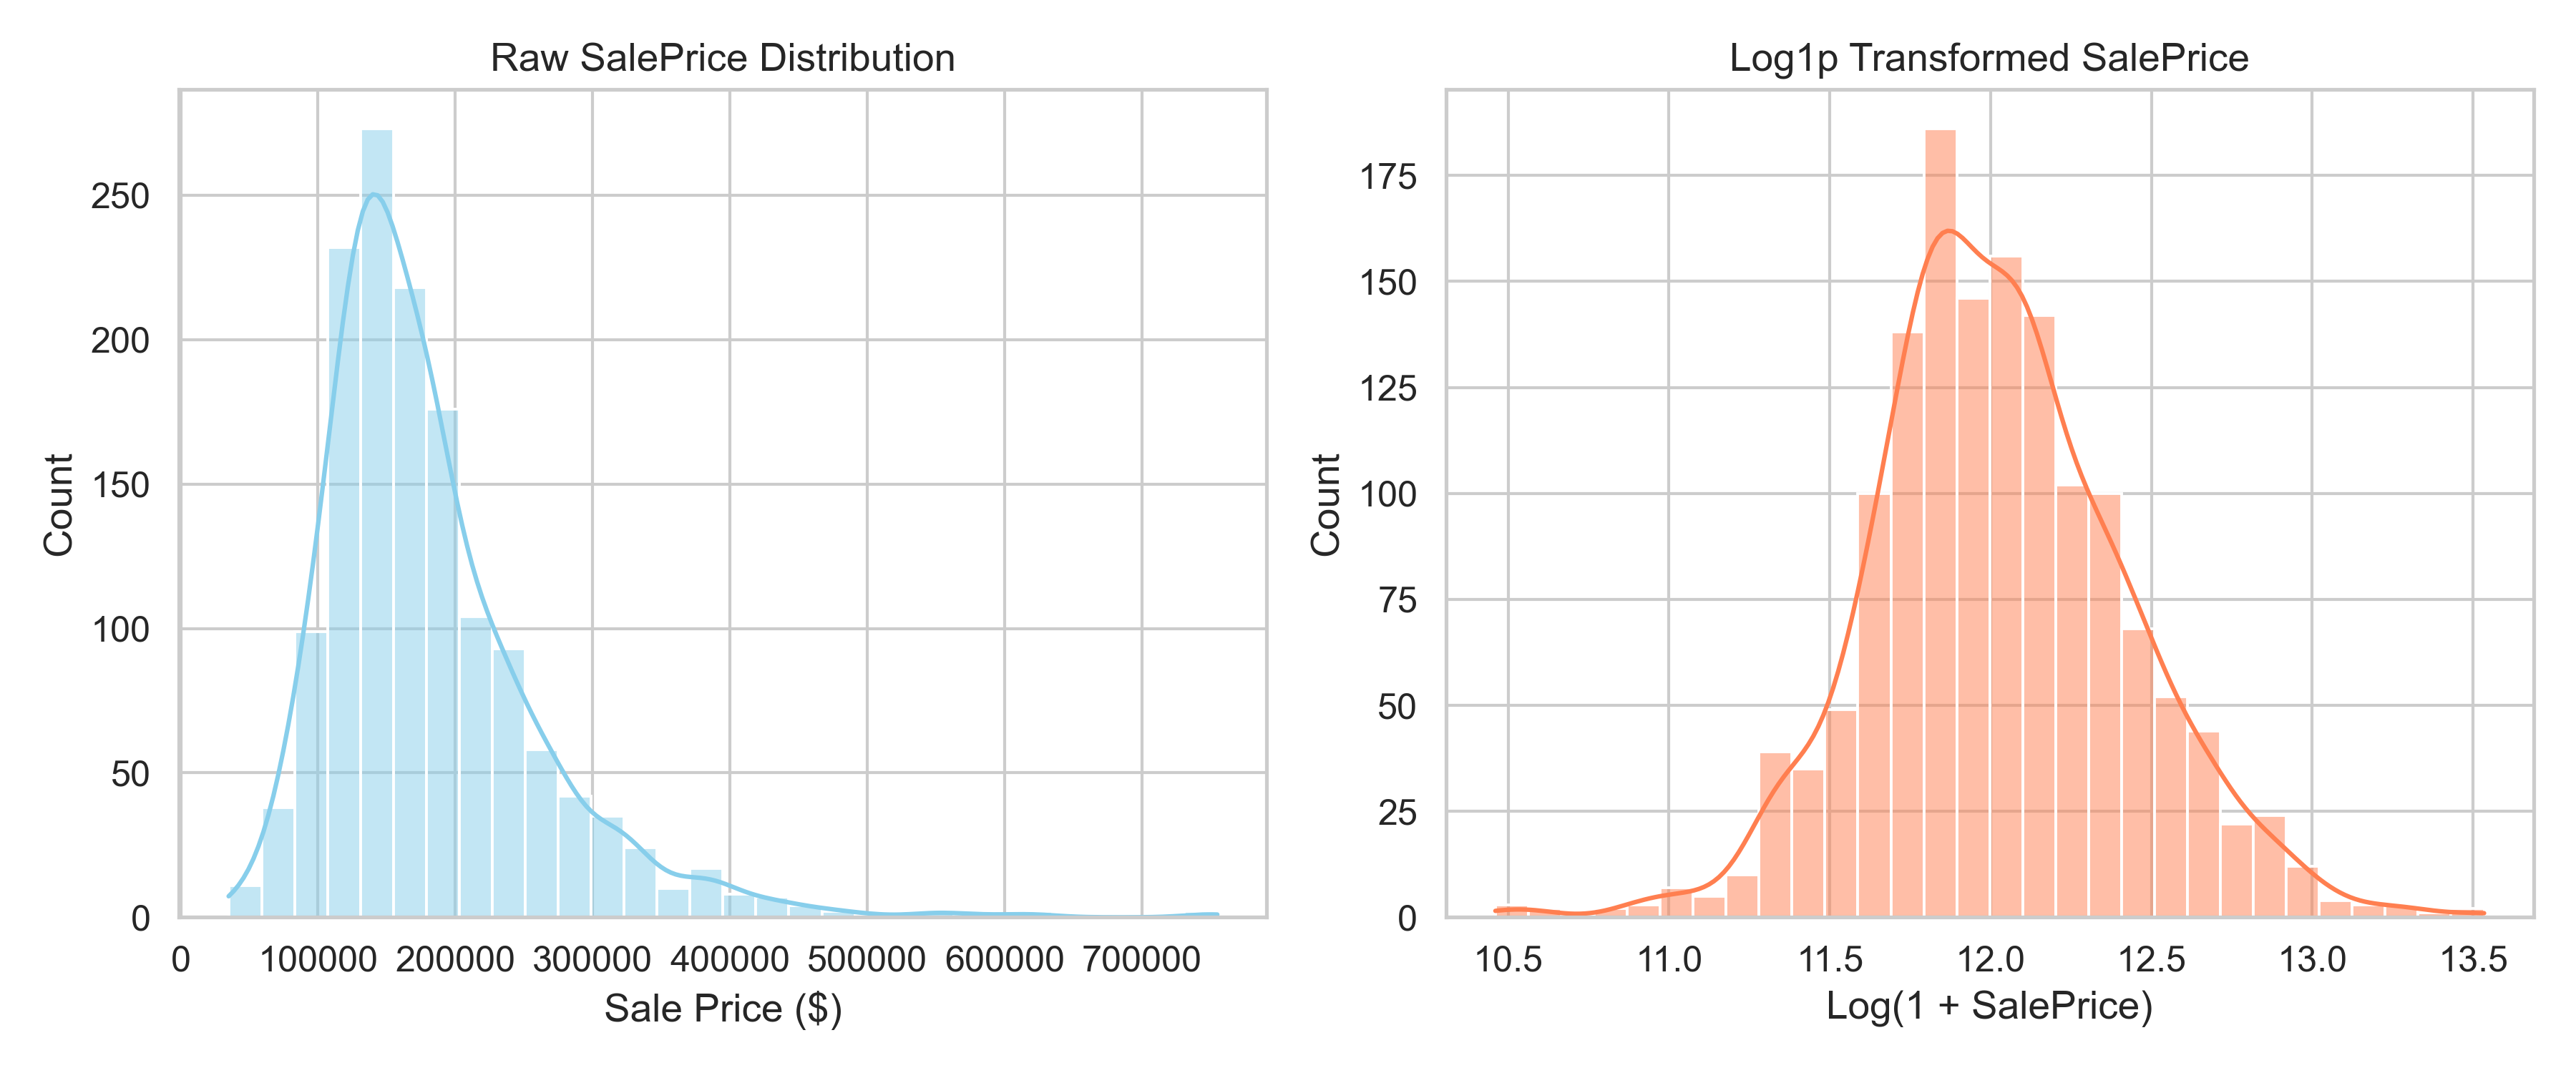
\includegraphics[width=\columnwidth]{../fig-saleprice-dist.png} 
 \caption{Distribution of Raw SalePrice vs Log1p-transformed SalePrice. High-value outliers pull the untransformed mean higher than the median.} \label{fig:saleprice}
\end{figure}

The dataset correlation heatmap (Fig. \ref{fig:corr}) highlighted strong positive correlations between price and features like \texttt{OverallQual}, \texttt{TotalSF}, and \texttt{GrLivArea}. However, it also uncovered multicollinearity (\texttt{GarageCars} and \texttt{GarageArea} share a correlation of $\sim 0.88$), necessitating regularized methodologies. 

\begin{figure}[H] 
 \centering
 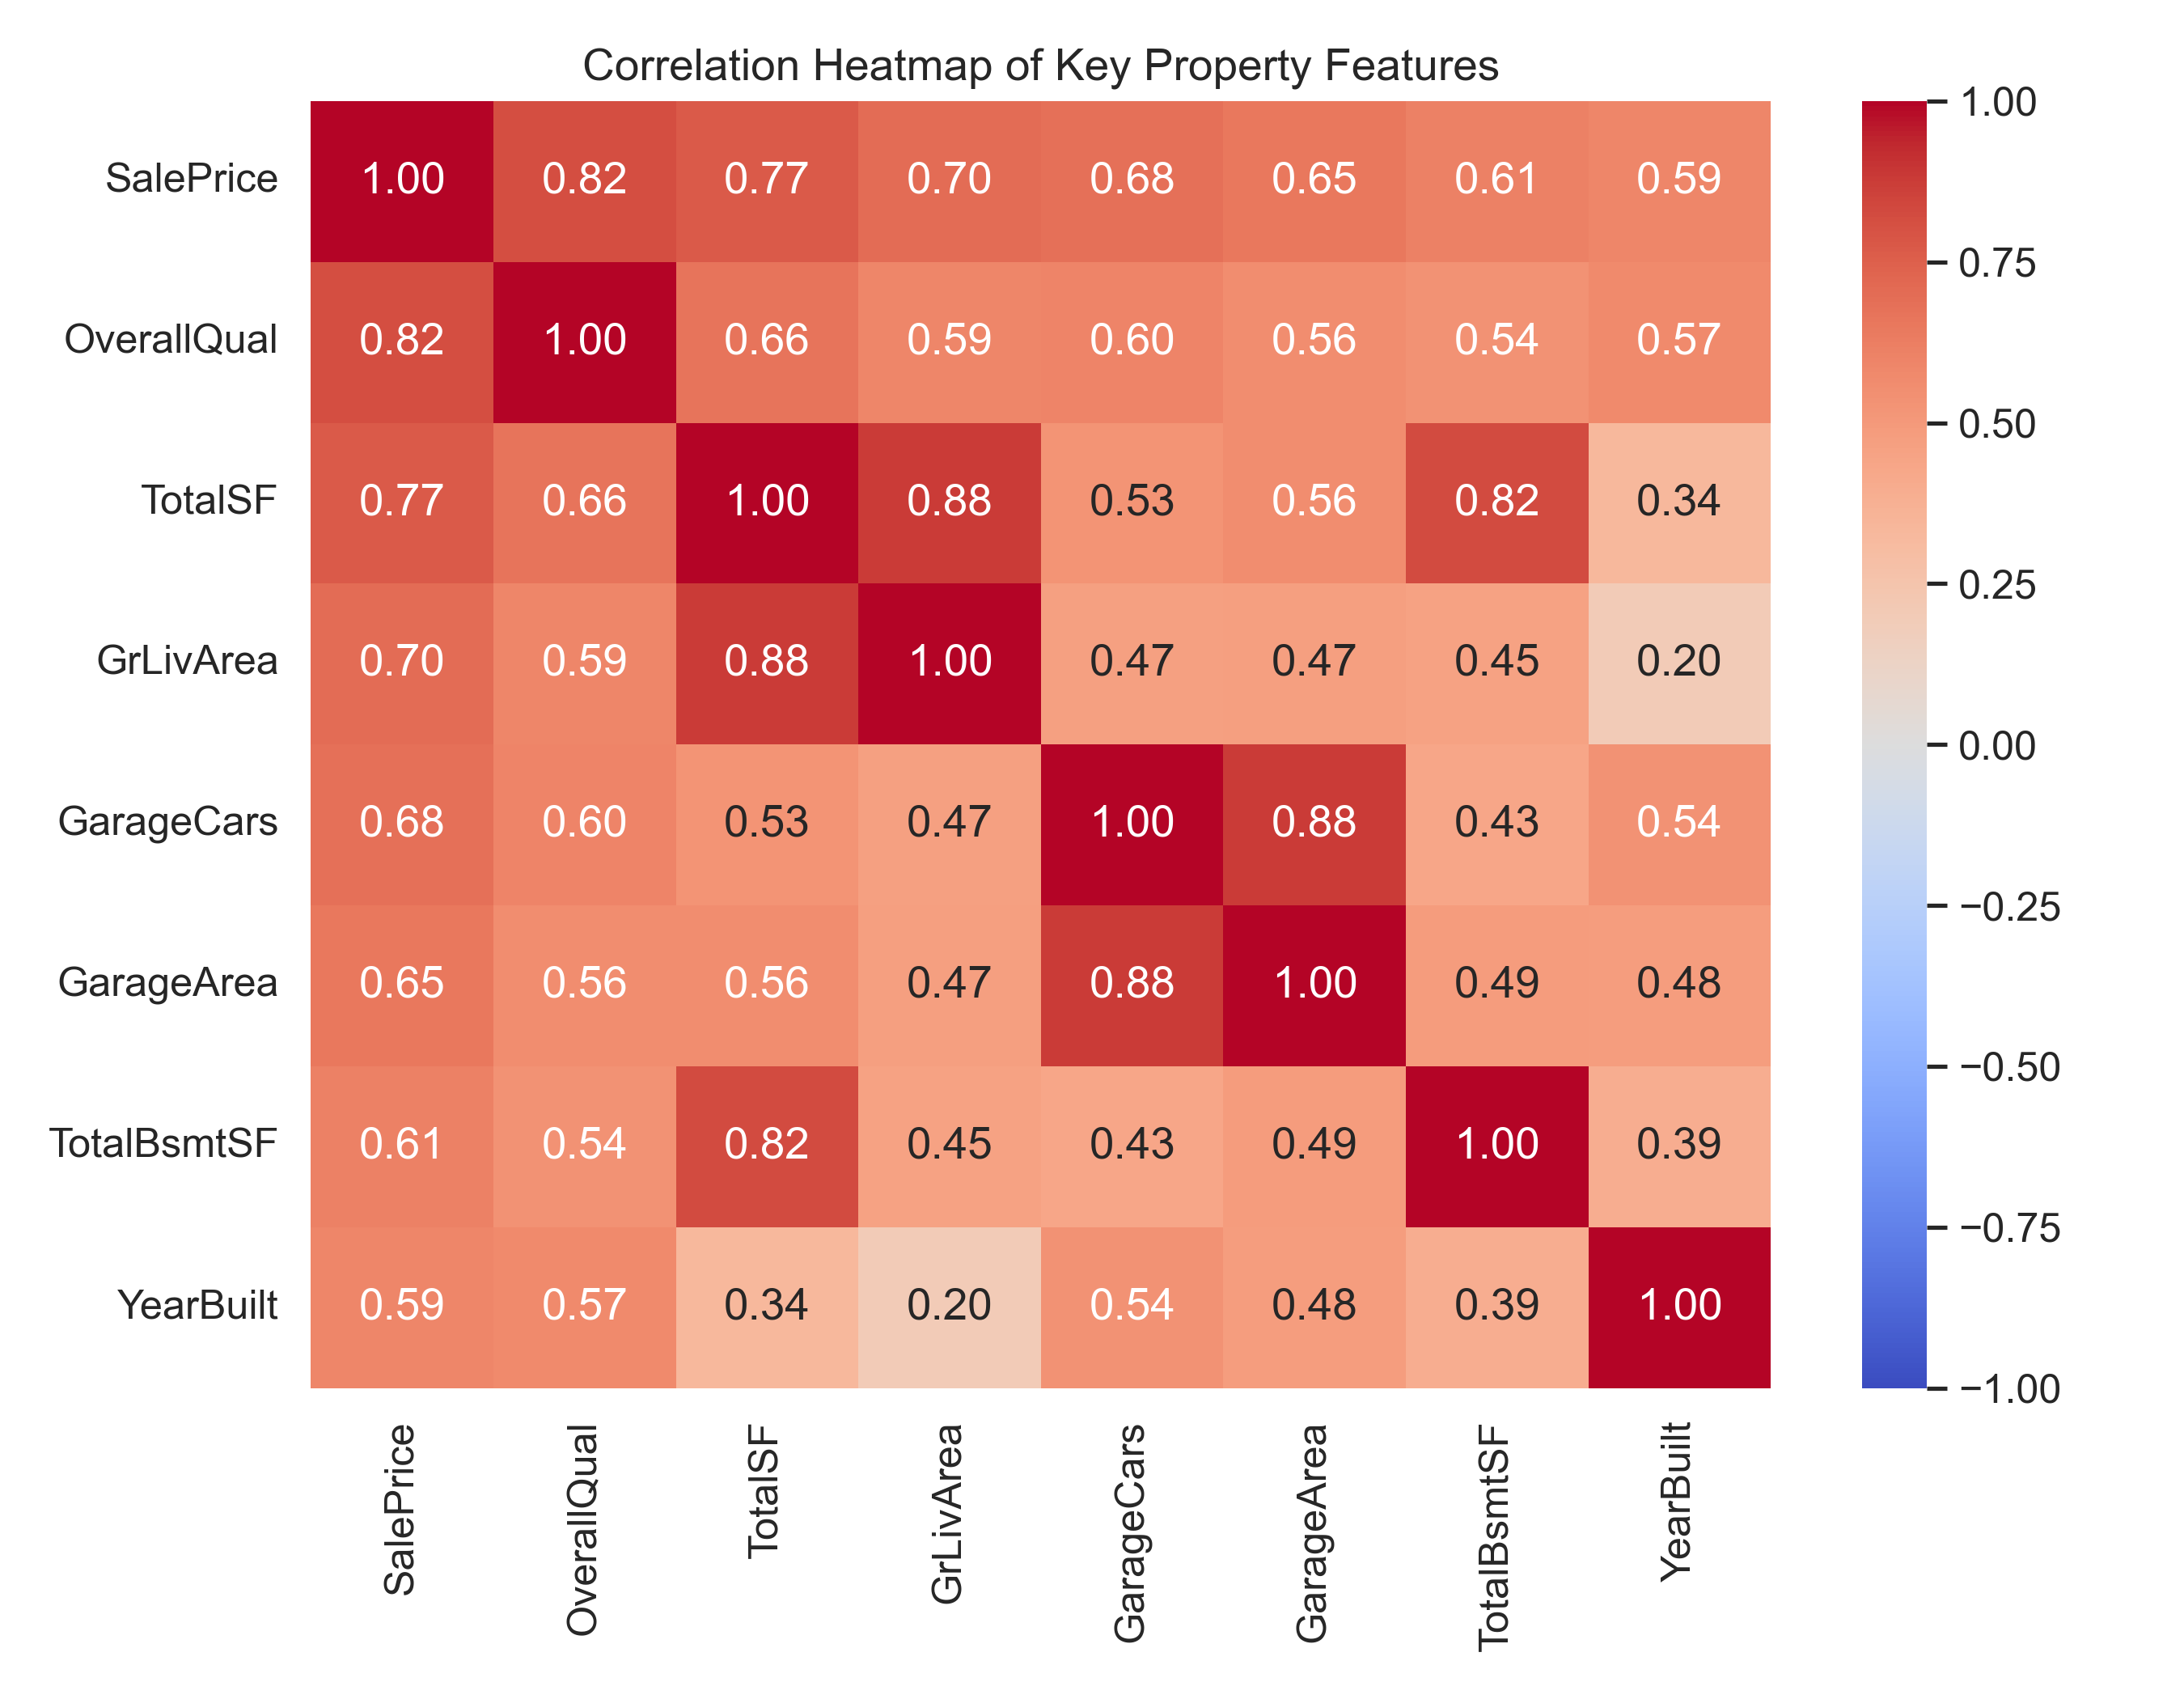
\includegraphics[width=\columnwidth]{../fig-correlation-matrix.png} 
 \caption{Correlation Heatmap of Key Property Features reveals high co-linearity among structural features.} \label{fig:corr}
\end{figure}

Additionally, outsized properties trading at oddly low values (Luxury Outliers) were spotted (Fig. \ref{fig:outliers}), verifying that specific anomalies can heavily bias linear fit lines without pre-processing.

\begin{figure}[H] 
 \centering
 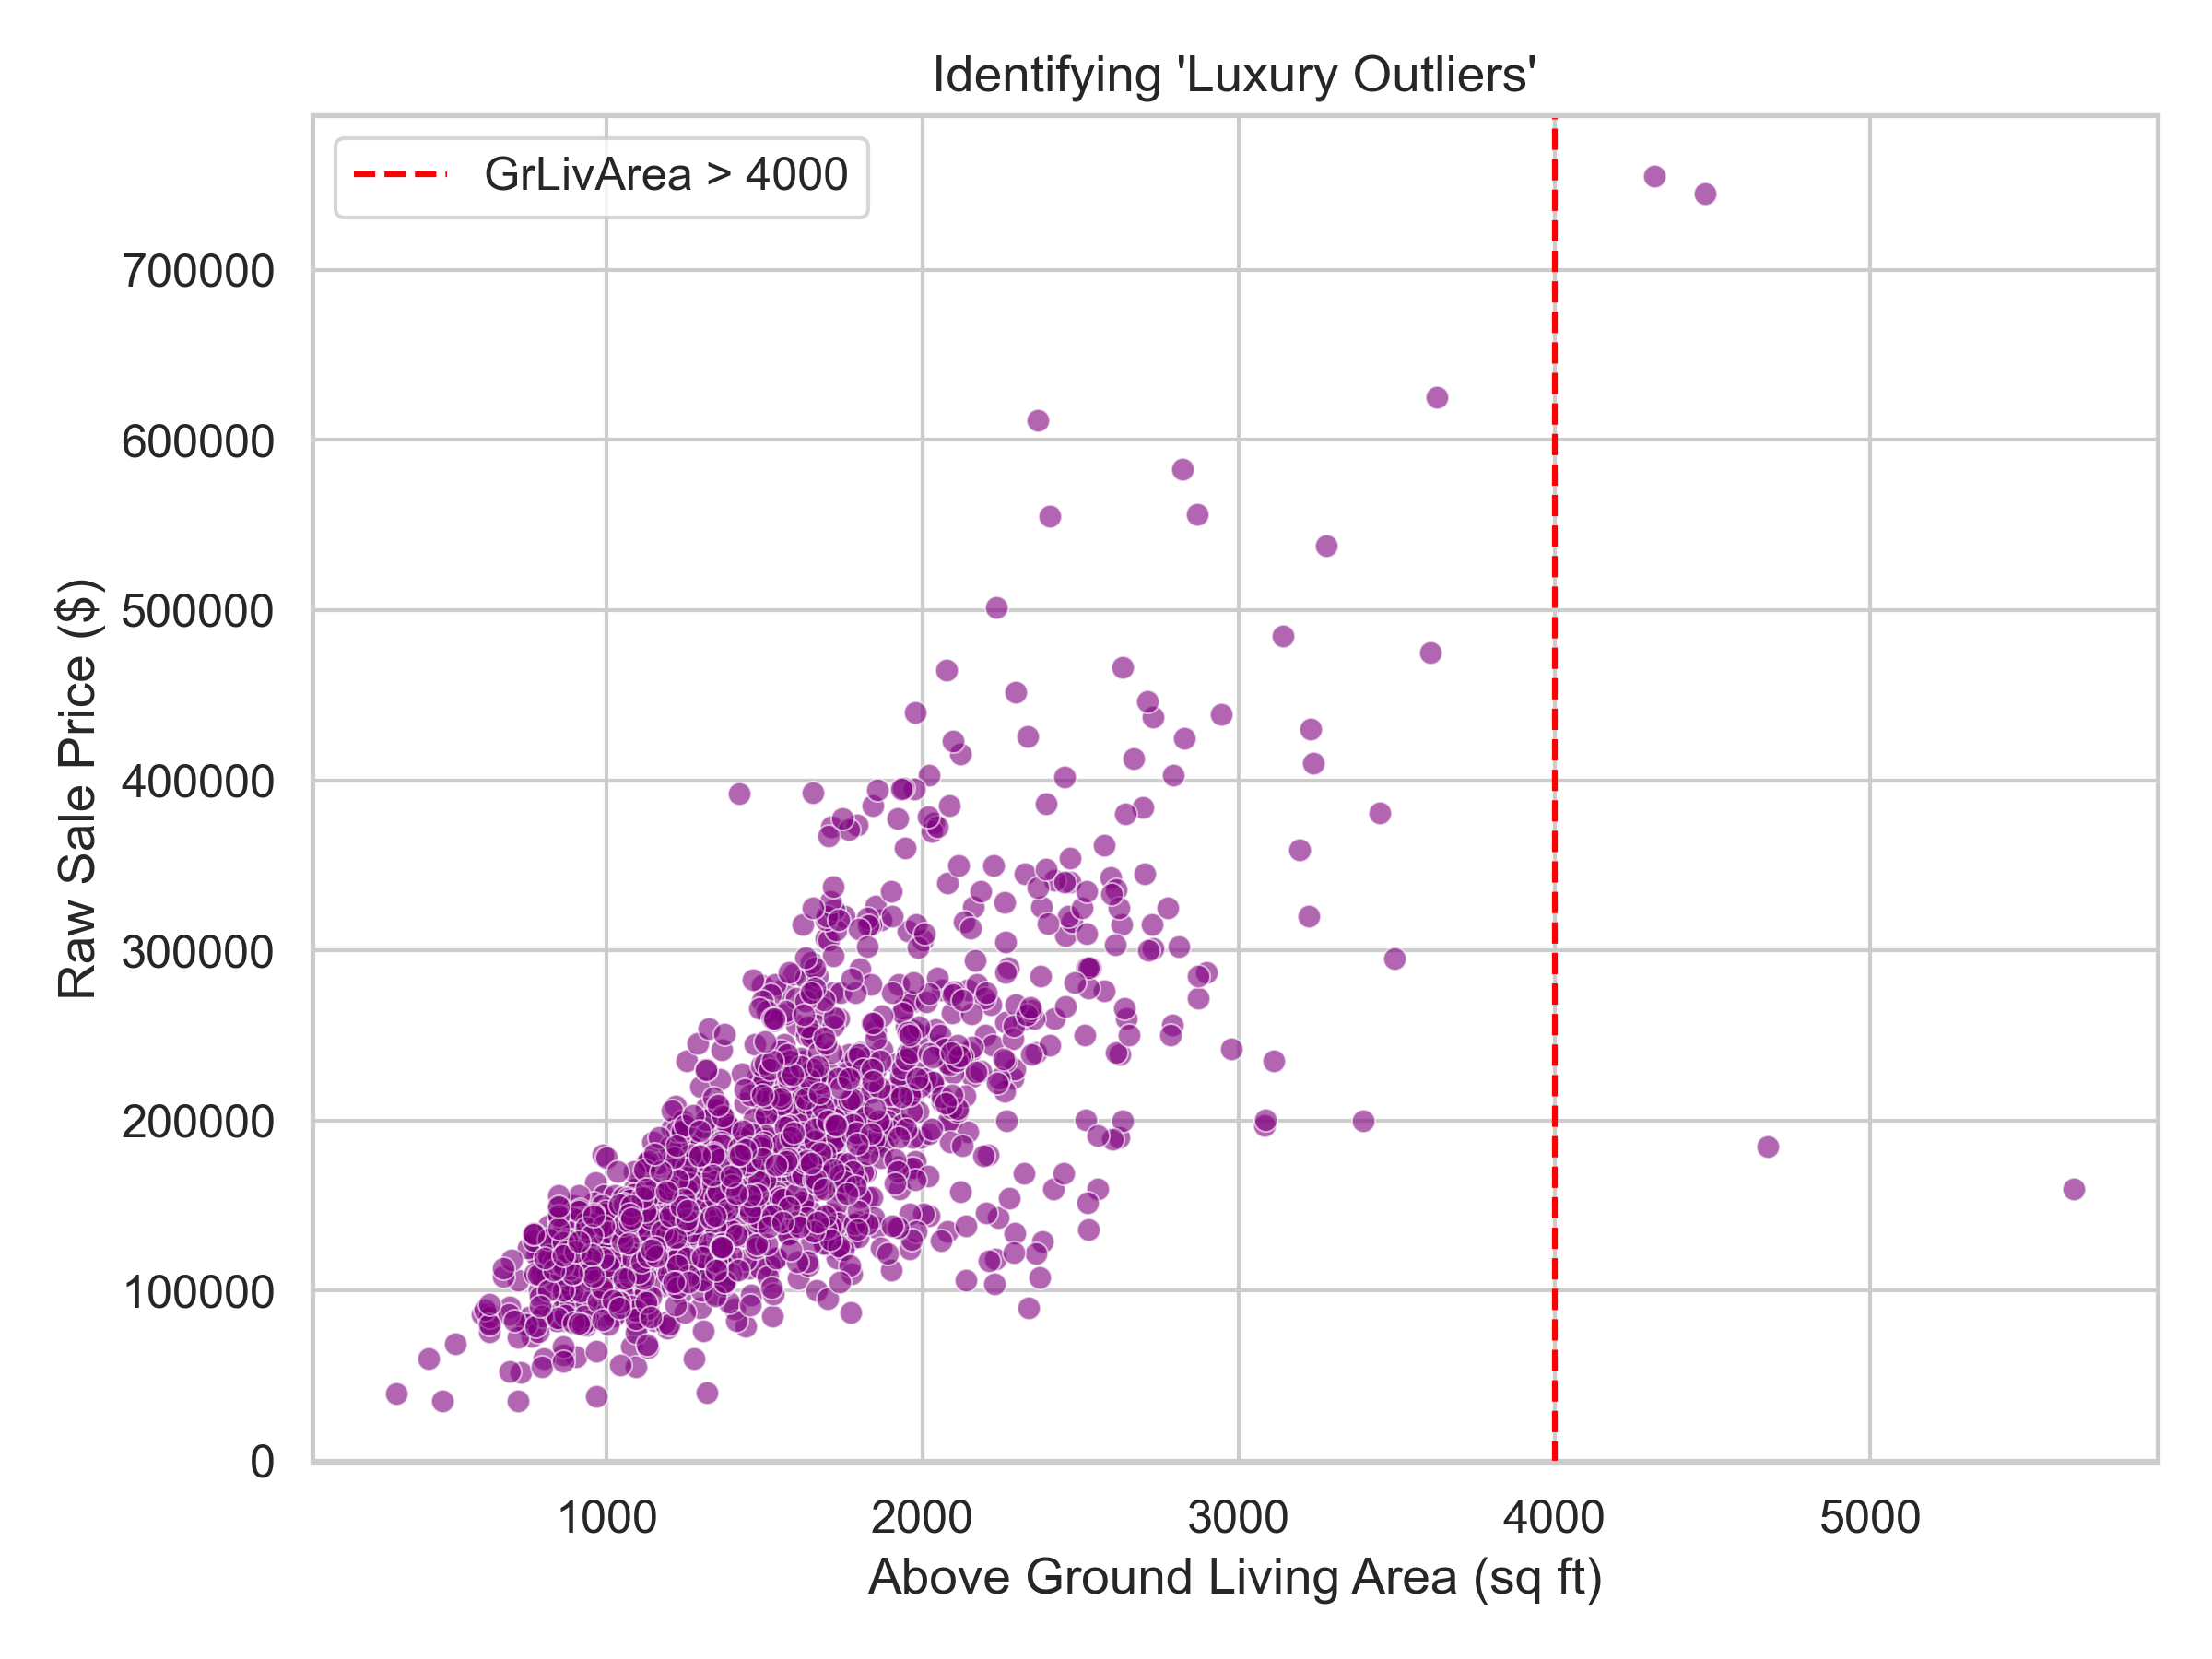
\includegraphics[width=\columnwidth]{../fig-outlier-detection.png} 
 \caption{Scatter Plot of Above Ground Living Area vs Raw SalePrice to Identify Outliers.} \label{fig:outliers}
\end{figure}

A spatial analysis visually reinforced the impact of neighborhoods like \texttt{NridgHt} and \texttt{StoneBr} which commanded massive price premiums (Fig. \ref{fig:neighborhoods}), while temporal plotting demonstrated a clear, non-linear pricing increase correlated to the property's original construction year (Fig. \ref{fig:year}).

\begin{figure}[H] 
 \centering
 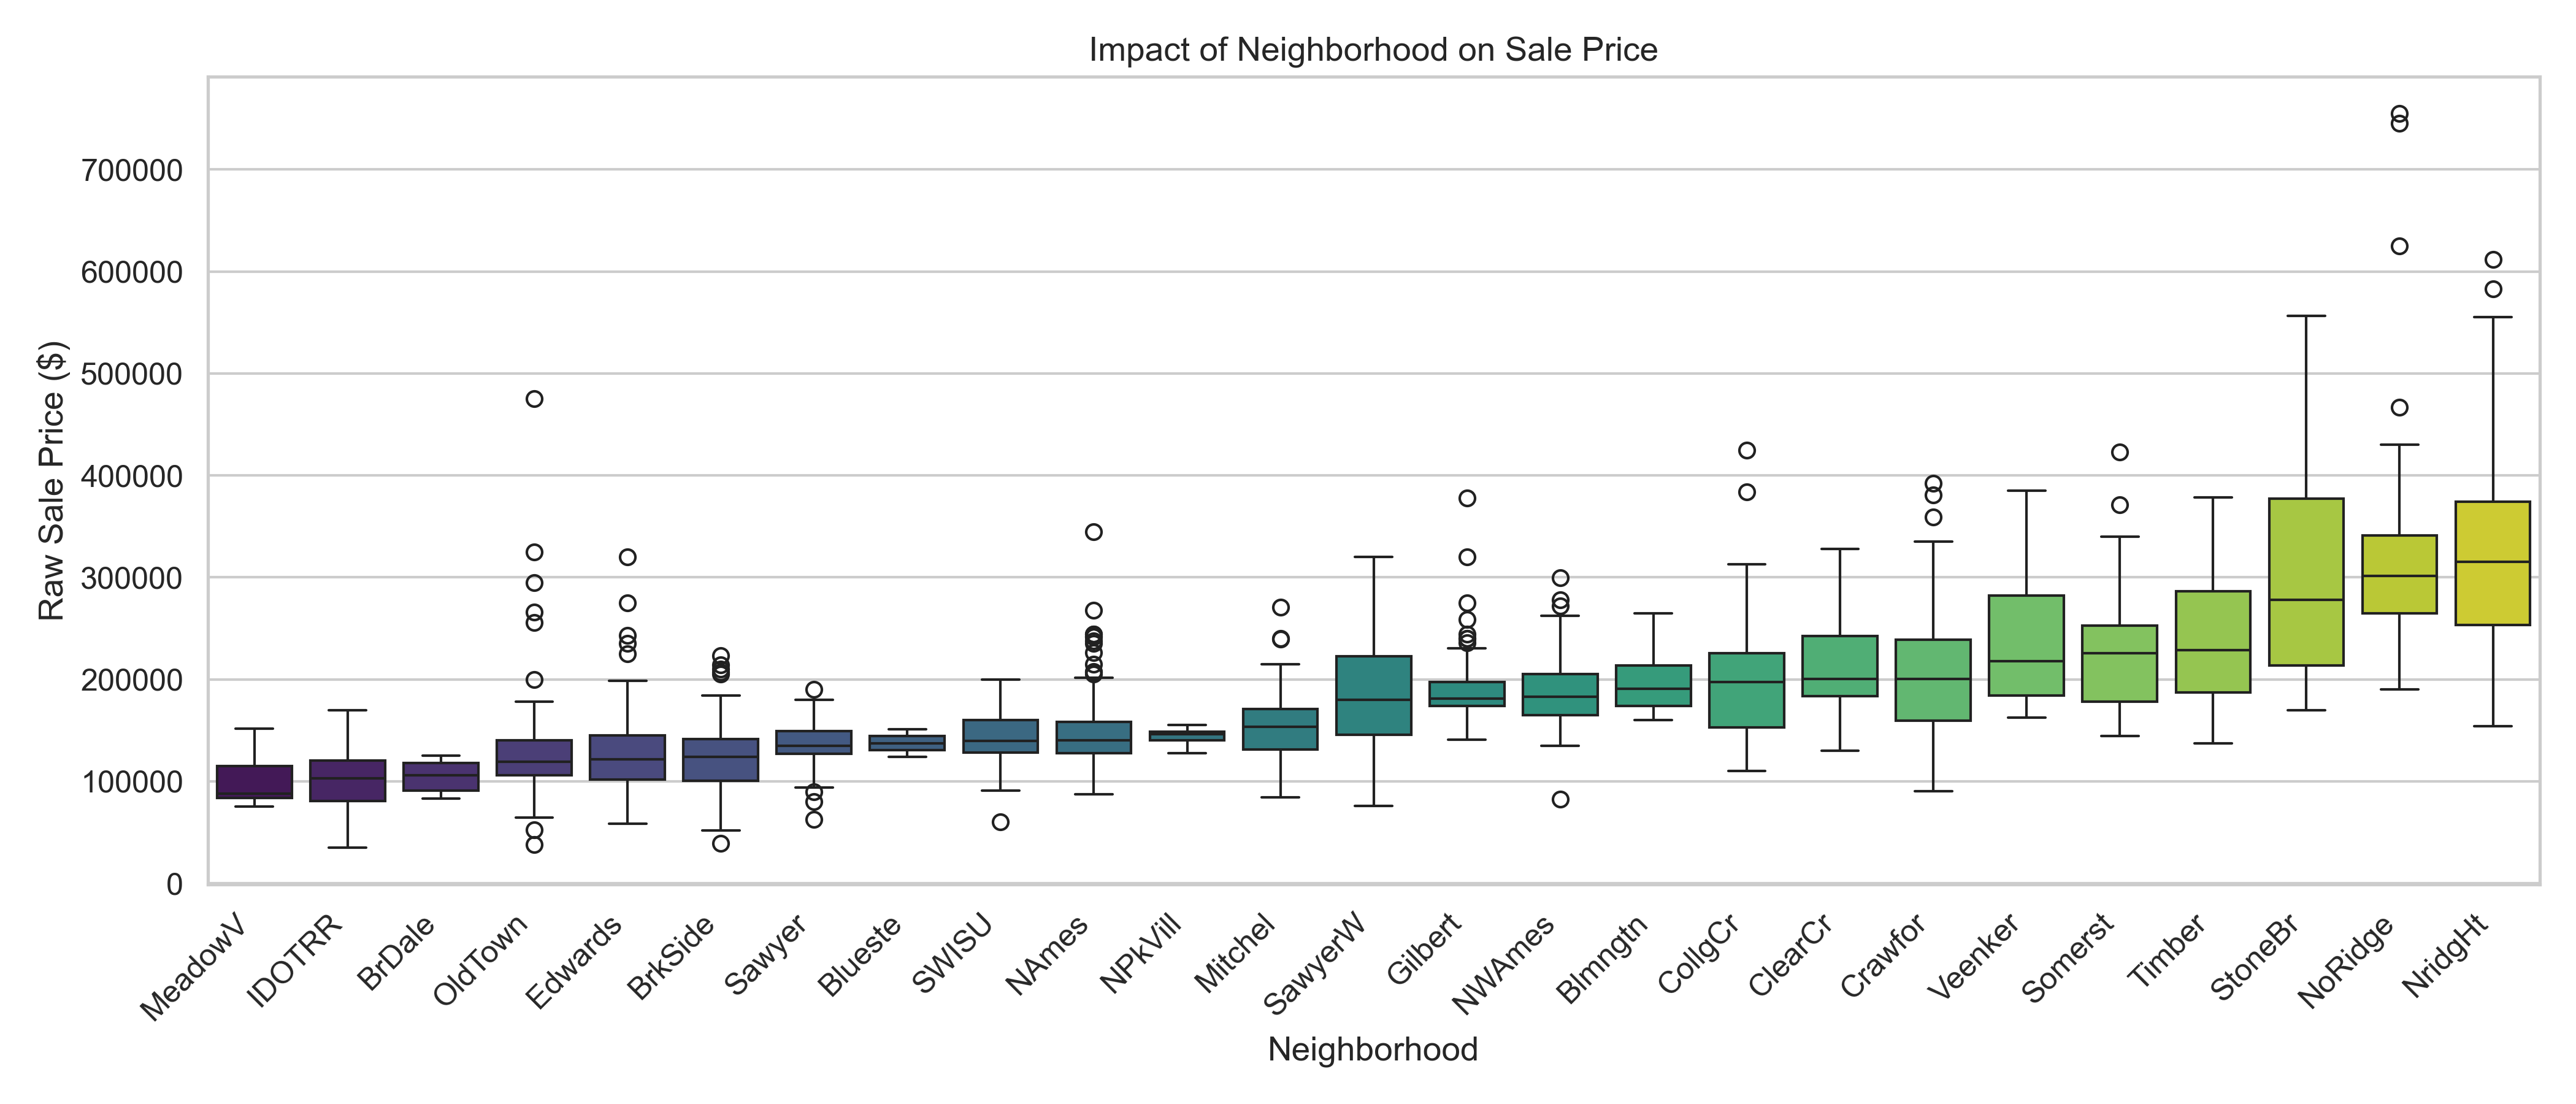
\includegraphics[width=\columnwidth]{../fig-neighborhood-price.png} 
 \caption{Sale Price Distribution by Neighborhood illustrating geographical price variance.} \label{fig:neighborhoods}
\end{figure}

\begin{figure}[H] 
 \centering
 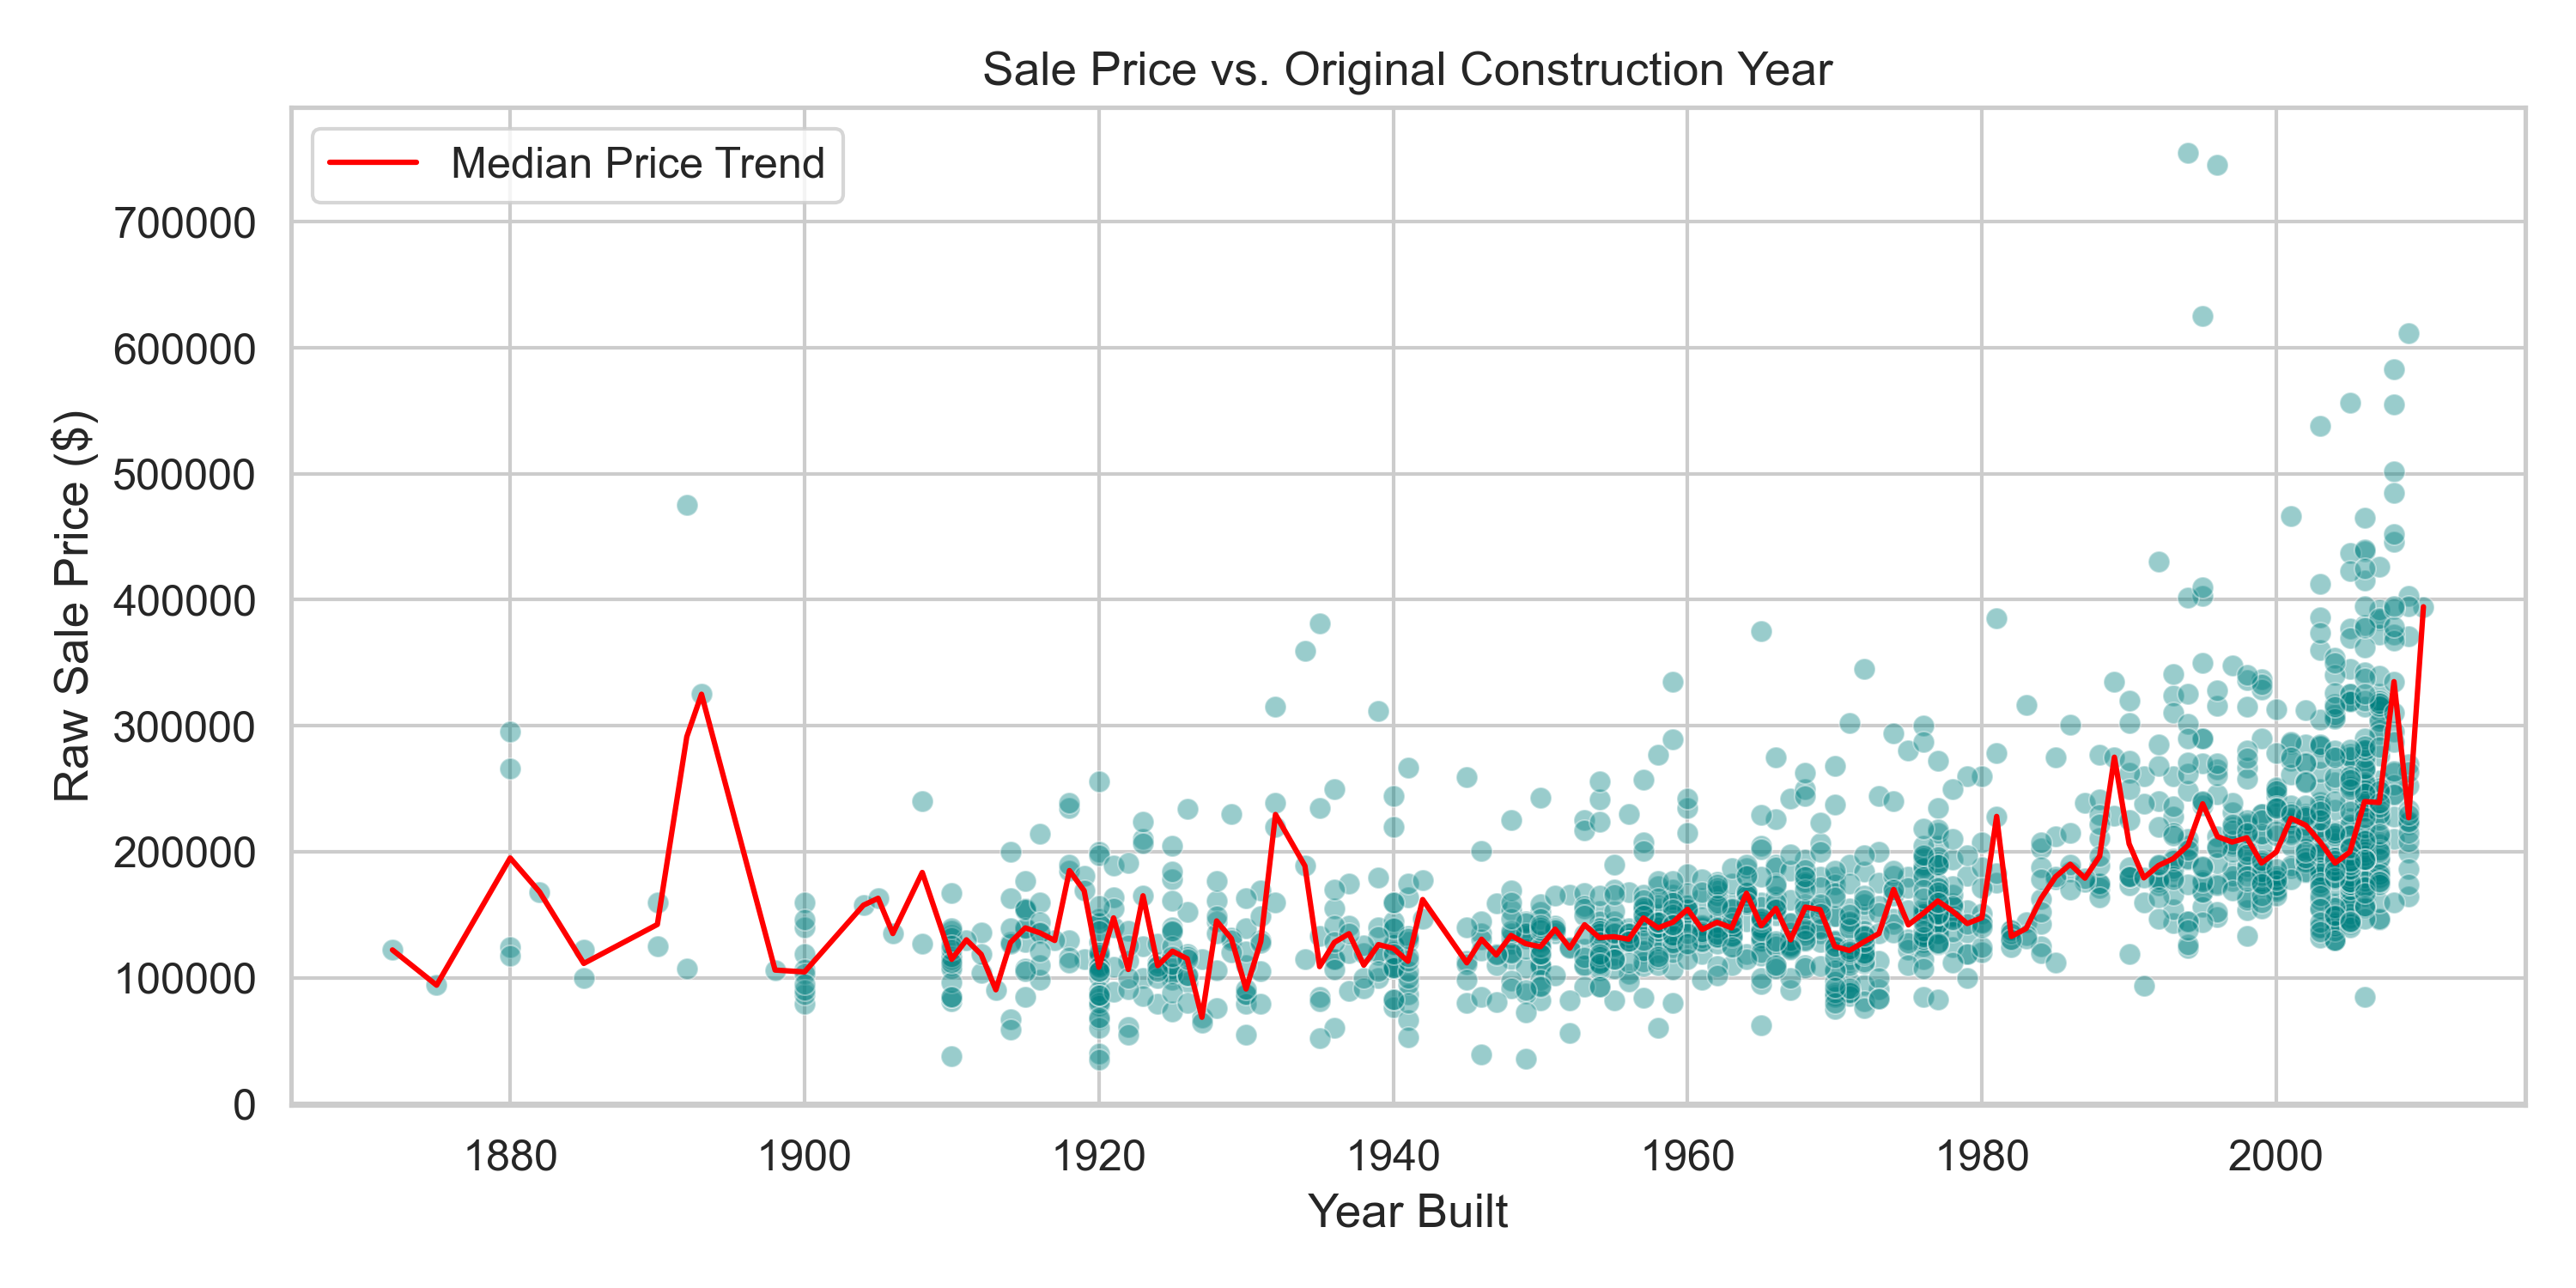
\includegraphics[width=\columnwidth]{../fig-year-built.png} 
 \caption{Impact of Year Built on Sale Price presenting a non-linear relationship between construction date and sale value.} \label{fig:year}
\end{figure}

\subsection{Market Segments}

The PCA successfully collapses quality and age indicators into a single ``Age-Quality Index'' axis. Plotting this against the log-transformed Sale Price revealed distinct Market Segments (Budget, Standard, Premium) clustered by K-Means, mathematically validating theoretical real-estate tiers.

\begin{figure}[H] 
 \centering
 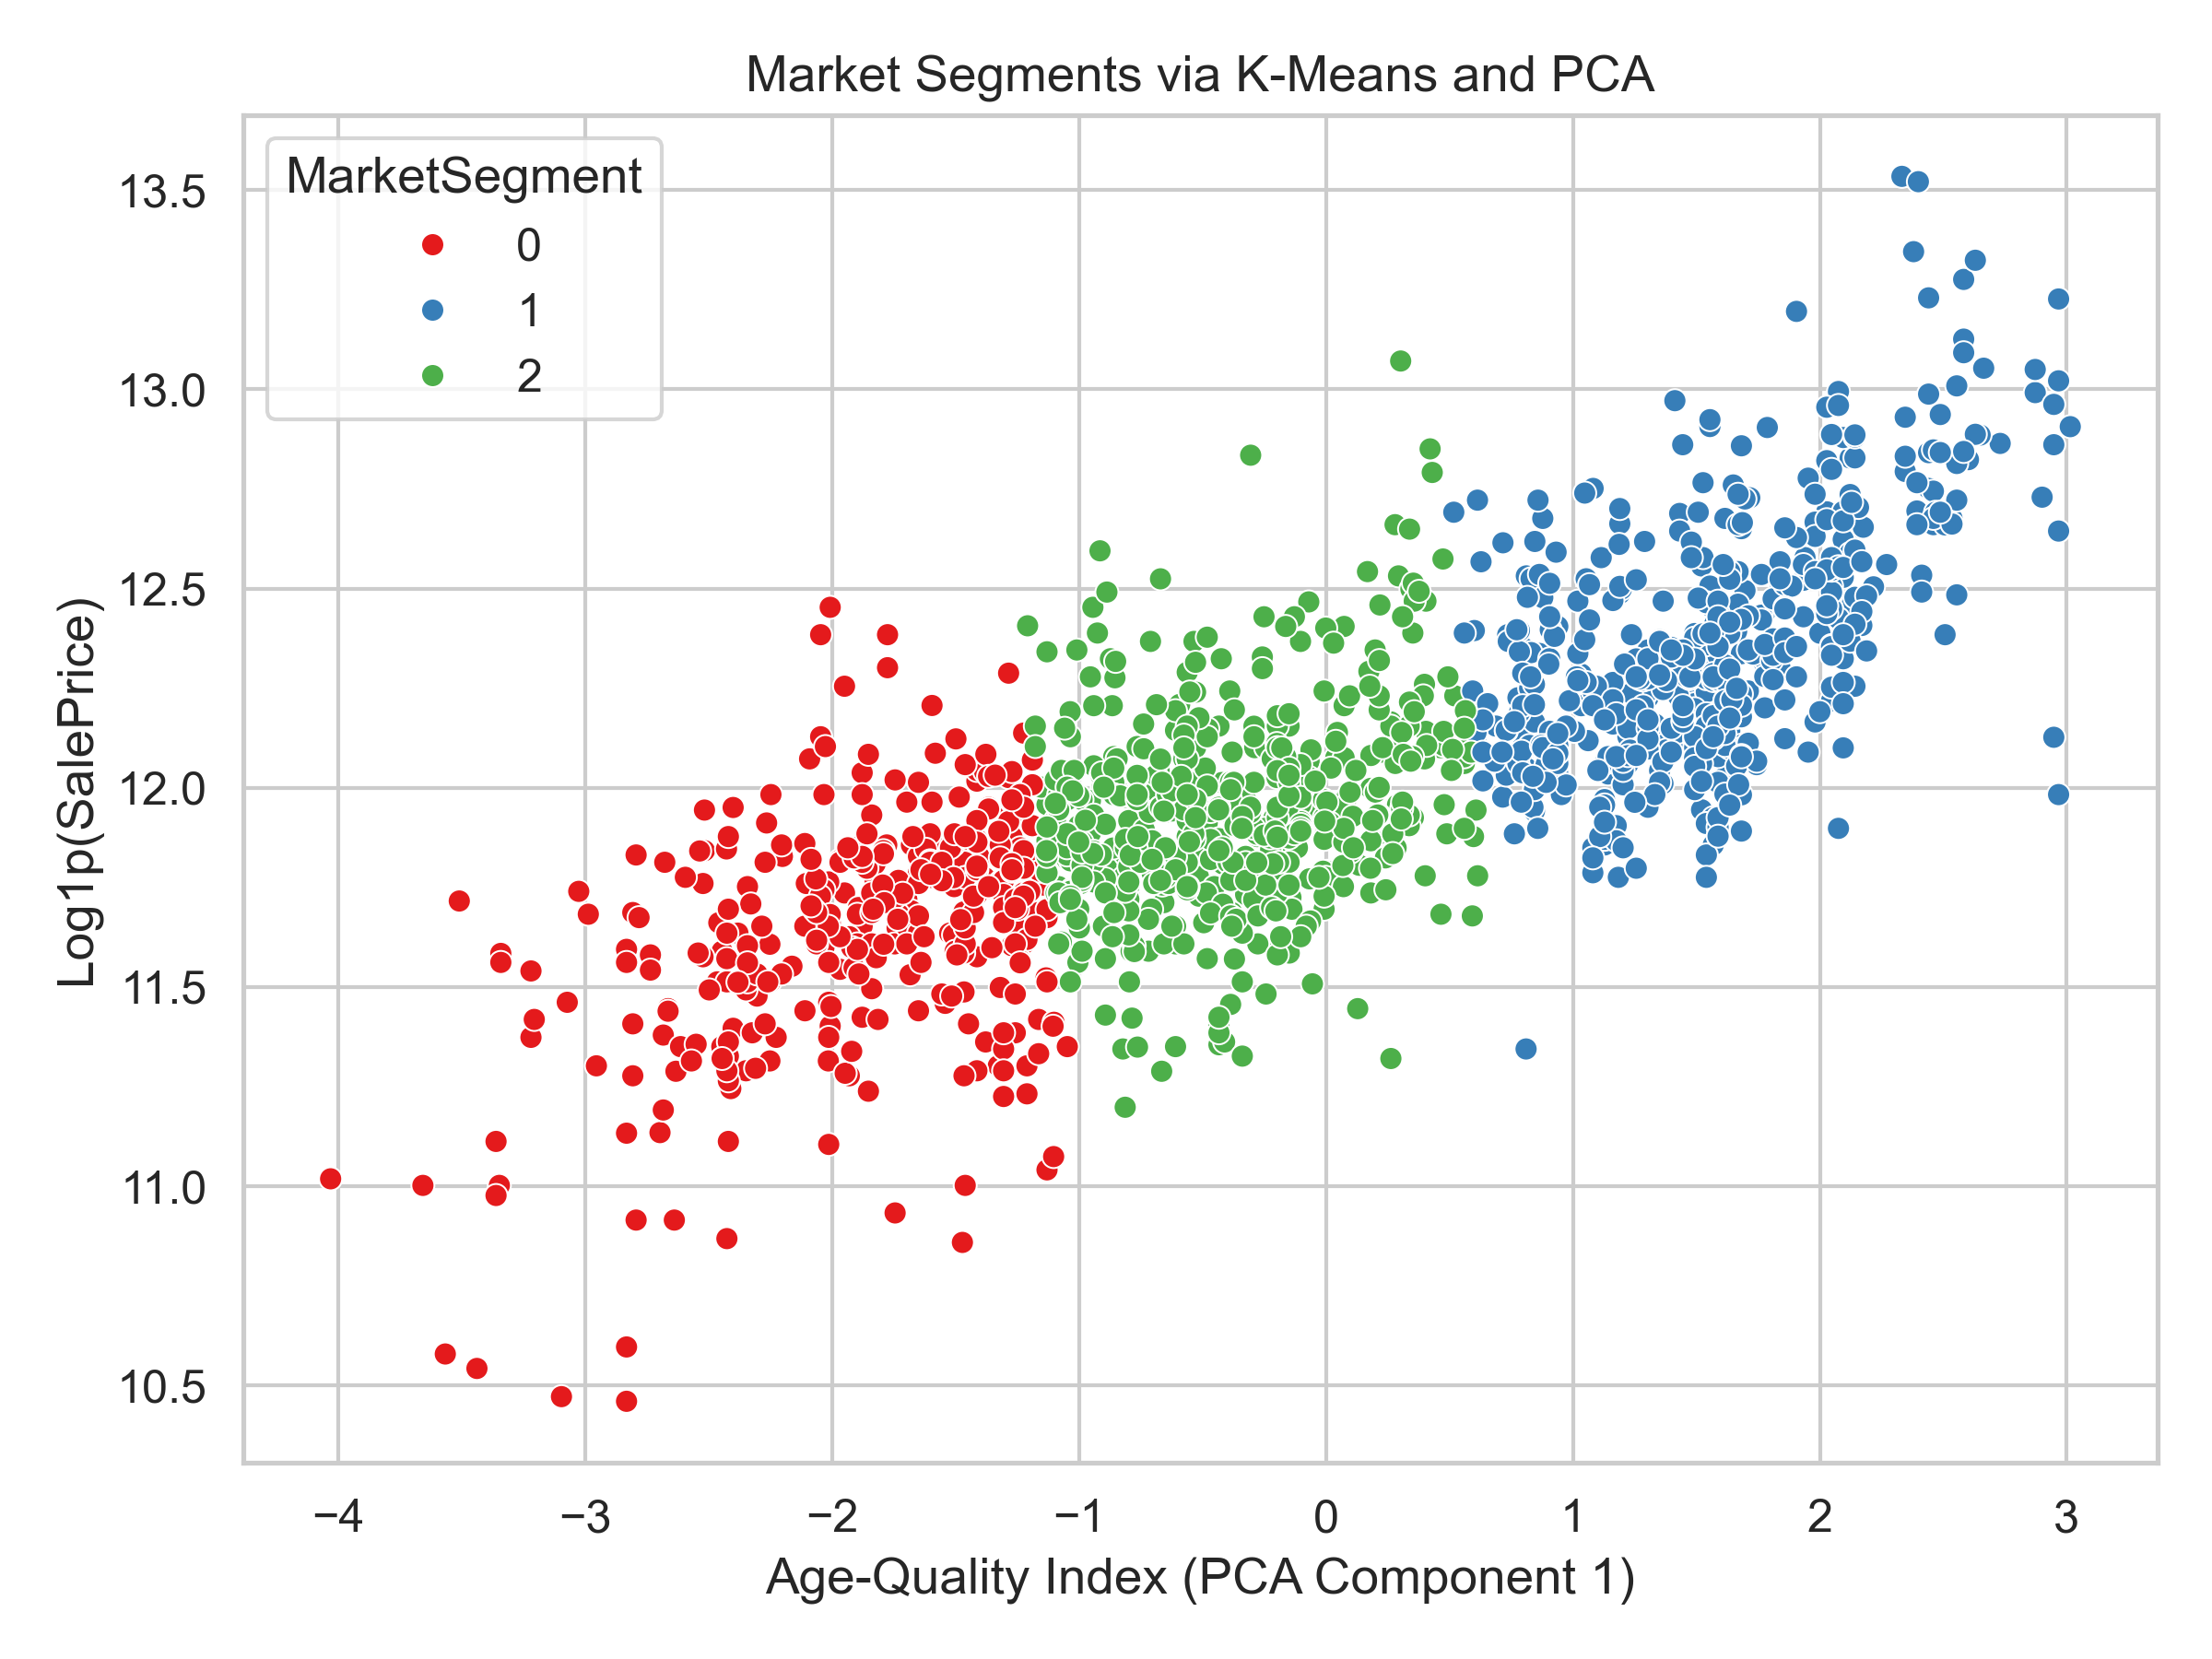
\includegraphics[width=\columnwidth]{../unsupervised-learning.png}
 \caption{Market Segments via K-Means and PCA showing Budget, Standard, and Premium clusters computed via unsupervised learning.} \label{fig:segments}
\end{figure}

\subsection{Predictive Performance}

Through building these machine learning pipelines, our findings highlight the power of regularization and ensemble tools.

\begin{table}[H]
 \caption{Advanced Regression Evaluation: Lasso vs. RF vs. XGBoost}
 \label{table-1}
 \centering
 \resizebox{\columnwidth}{!}{
 \begin{tabular}{lc} \toprule
  \textbf{Model} & \textbf{CV RMSE (Log scale)} \\ \midrule
  Lasso Regression (Tuned) & 0.201 \\
  Random Forest & 0.169 \\
  XGBoost (Ensemble) & \textbf{0.163} \\
  \bottomrule
 \end{tabular}}
\end{table}

As shown in Table~\ref{table-1}, Lasso Regression proved highly effective at handling multicollinearity by driving the coefficients of redundant features to zero. However, XGBoost and Random Forest consistently outperformed the linear baseline. The ensemble models dynamically mapped complex spatial and contextual interactions, yielding the lowest RMSE scores on the test folds. Addressing the skewed distribution through Log transformations confirmed that modeling performance was structurally preserved without being corrupted by luxury outliers.

\section{Conclusion}

Our comprehensive analysis of the Ames Housing dataset successfully transformed raw property attributes into robust, predictive insights. By rigorously addressing structurally missing variables and engineering aggregated features like \texttt{TotalSF}, we established a highly refined foundation. Critically, we mitigated the severe right-skewness inherent in real estate pricing by applying a Log(1p) transformation to the sale price. 

To answer our primary research question, our comparative findings are unequivocal. While Regularized Linear Regression (LassoCV) performed admirably by isolating fundamental value drivers, it ultimately hit a performance ceiling. Advanced ensemble learners, specifically Random Forest and XGBoost, consistently outperformed the linear baseline minimizing the Cross-Validated RMSE. Ensemble algorithms organically mapped this intricate, multidimensional hedonic landscape without requiring exhaustive manual interaction engineering. 

Future enhancements should expand beyond immediate structural parameters. Integrating macroeconomic indicators or utilizing geospatial APIs to calculate exact proximity to high-value amenities could capture stylistic premiums that standard tabular datasets fundamentally struggle to quantify.

\section*{Acknowledgments}
We acknowledge Kaggle for providing the primary Ames Housing datatset and the academic community associated with quantitative real estate economics framework for fundamental evaluation strategies.

% Bibliographic references
\bibliographystyle{IEEEtran}
\bibliography{References}

\end{document}
